\documentclass[12pt,a4paper,titlepage]{article}
\usepackage[utf8]{inputenc}
\usepackage{polski}
\usepackage{graphicx}
\usepackage{tikz}
\usepackage{pgfplots}
\usepackage{pgfgantt}
\usepackage{xcolor}
\usepackage{floatrow}
\usepackage{minted}
\usepackage{amsmath}
\usepackage{caption}
\usepackage{url}
\usepackage[nottoc,numbib]{tocbibind}

\pgfplotsset{compat=1.16}
 
\setminted{
    linenos=true,
    autogobble,
    breaklines,
    frame=lines,
    framerule=1pt,
    framesep=10pt,
    fontsize=\small
}

\newenvironment{longlisting}{}{}
% \renewcommand\listingscaption{Listing}
\renewcommand\listoflistingscaption{Spis listingów}
% \renewcommand\figurename{Rys.}

\makeatletter
\newcommand{\linia}{\rule{\linewidth}{0.4mm}}
\renewcommand{\maketitle}{\begin{titlepage}
    \begin{center}\small
    \huge{\textsc{Politechnika Wrocławska\\
    Wydział Elektroniki}}\\\linia
    \end{center}
    \vspace{2cm}
    \noindent
    \begin{center}
        \LARGE{Zarządzanie w systemach i sieciach komputerowych - projekt}\vspace{2cm}
        
        \LARGE \textbf{\@title}
            \end{center}
    
    \vspace{2cm}
    \begin{minipage}{5cm}
        \textsc{Autor:}\\
            \@author
    \end{minipage}
    \hfill
    \begin{minipage}{6.5cm}
        \textsc{Prowadzący zajęcia:}\\
        Dr inż. Robert Wójcik, W4/K-9
    \end{minipage}
    
    \vspace*{1cm}
    \begin{flushright}
        \begin{minipage}{6.5cm}
        \textsc{Ocena pracy:}
    \end{minipage}
    \end{flushright}
    
    \vspace*{\fill}
    \begin{center}
    \linia\newline
    \large{\textsc{Wrocław, \the\year}}
    \end{center}
  \end{titlepage}%
}
\makeatother
\author{Marcin Jasiński, 235559\\
        Justyna Skalska, 225942}
\title{Równoległa kompresja plików tekstowych z wykorzystaniem rdzeni CUDA karty graficznej}

\begin{document}
\maketitle
\tableofcontents
\newpage

{
\let\oldnumberline\numberline
\renewcommand{\numberline}{\figurename~\oldnumberline}
\listoffigures
}
\newpage

{
\let\oldnumberline\numberline
\renewcommand{\numberline}{\tablename~\oldnumberline}
\listoftables
}
\newpage

\addcontentsline{toc}{section}{\listoflistingscaption}
{
\let\oldnumberline\numberline
\renewcommand{\numberline}{\listingname~\oldnumberline}
\listoflistings
}
\newpage

\floatsetup[listing]{style=Plaintop}
\floatsetup[table]{style=Plaintop}

%-------------------------------------------------------------------------
\section{Wstęp}
\subsection{Cel projektu}
% Co było oczekiwanym rezultatem pracy?
Celem projektu było opracowanie, a następnie implementacja algorytmu kompresji plików opartego na autorskim pomyśle. Wykorzystanie implementacji opracowanego algorytmu, w postaci możliwej do uruchomienia i wykorzystującej rdzenie CUDA~\cite{cuda} karty graficznej GeForce serii 900~\cite{geforce-900-series}, znajdującej się na wyposażeniu komputera oraz przeprowadzenie testów w zakresie zmierzenia poziomu efektywności działania algorytmu (poziom kompresji) oraz czasu wykonania się procesu kompresji plików.

\subsection{Zakres projektu}
% Co trzeba było zrobić, aby ten rezultat osiągnąć?
Zakres projektu przewidywał implementację autorskiego algorytmu kompresji przy użyciu biblioteki JCuda~\cite{jcuda} oraz języka Java, z którego każde z nas korzysta na co dzień. Dzięki temu implementacja była dla nas znacznie łatwiejsza niż przy wykorzystaniu języka C lub C++. Testy miały zostać wykonane na jednym z naszych komputerów posiadającym kartę NVIDIA GeForce 940MX.~\cite{gtx-940mx}

%-------------------------------------------------------------------------
\section{Sformułowanie problemu}

\subsection{Podstawowe założenia}
Problem równoległej kompresji rozwiązywany będzie przy uwzględnieniu następujących założeń:
\begin{itemize}
    \item Kompresowane będą duże pliki tekstowe (o rozmiarze przekraczającym 50MB),
    \item Kompresja odbywać się będzie przy wykorzystaniu obliczeń równoległych na rdzeniach CUDA karty graficznej znajdującej się na wyposażeniu komputera,
    \item Na podstawie zawartości pliku tekstowego tworzony będzie słownik, wykorzystywany w późniejszym etapie,
    \item Ze względu na specyfikę problemu, zakłada się ograniczenie liczby znaków w słowniku do 128.
\end{itemize}

\subsection{Opis wariantów problemu}

\subsubsection{Problem optymalizacyjny}
% TODO - dodać opis problemu
Problem optymalizacyjny polegał na dobraniu odpowiedniej liczby wątków uruchamianych równolegle tak, aby zmaksymalizować wydajność czasową kompresji.

\subsection{Zastosowany algorytm}
Zastosowany algorytm został zaproponowany przez doktora Dominika Żelaznego, jako uproszczony model kompresji plików tekstowych, bazujący na kompresji Huffmana~\cite{kompresja-huffmana}, jednak z pominięciem etapu sortowania znaków w słowniku względem częstości występowania i tworzenia drzewa. W pierwszym etapie przeglądany jest cały plik tekstowy oraz odnotowywane jest wystąpienie każdego nowego znaku, niebędącego dotychczas umieszczonym w słowniku. Następnie na podstawie długości słownika (liczby poszczególnych znaków w tekście) określana jest minimalna liczba bitów potrzebna do zakodowania całego słownika. Na jej podstawie przekształca się źródłowy plik tekstowy, zamieniając każdy ze znaków w tekście na sekwencję bitową. Następnie, grupując symbole 0 i 1 w grupach po osiem, zamienia się je na wartości znakowe, a nowo utworzony plik zapisuje na dysku. 

\subsection{Analiza złożoności obliczeniowej algorytmu}
Ze względu na specyfikę algorytmu niemożliwe jest precyzyjne określenie złożoności obliczeniowej algorytmu. W szczególności algorytmy kompresji plików w formie wielowątkowej wykazują logarytmiczną złożoność obliczeniową. 

%-------------------------------------------------------------------------
\newpage
\section{Projekt aplikacji}
\subsection{Wykorzystane technologie i narzędzia projektowania}
Podczas tworzenia projektu wykorzystane zostały podane poniżej technologie oraz narzędzia:
\begin{itemize}
    \item OpenJDK 11~\cite{openjdk-11},
    \item Apache Maven 3.6.3~\cite{maven},
    \item JCuda 10.1.0~\cite{jcuda},
    \item IntelliJ IDEA 2019.3~\cite{intellij-idea},
    \item C~\cite{c-standard},
    \item Zestaw narzędzi CUDA.~\cite{cuda-toolkit-documentation}
\end{itemize}

\subsubsection{Specyfikacja techniczna karty graficznej}
Do testów wybrana została karta graficzna GeForce 940MX, która znajdowała się na wyposażeniu jednego z naszych komputerów. Jest to popularna w laptopach karta grafiki oparta na architekturze Maxwell, która pojawiła się w I połowie 2016 roku. Jest to układ wydajniejszy od układów zintegrowanych używanych w procesorach Intela, ale dużo słabszy od kart grafiki stosowanych w laptopach do gier. Ma 64-bitową szynę danych. Występuje w wersjach z pamięcią VRAM DDR3 i GDDR5. Wersja z pamięcią GDDR5 jest o ponad 1/3 wydajniejsza.~\cite{gtx-940mx}

\begin{table}[H]
\centering
\caption{Specyfikacja GeForce GTX940MX}
\begin{tabular}[H]{|p{4.5cm}|p{7.5cm}|}
\hline
\textbf{Producent} & NVIDIA \\
\hline
\textbf{Rodzina} & GeForce 900M \\
\hline
\textbf{Nazwa robocza} & N16S-GTR-B/S \\
\hline
\textbf{Architektura} & Maxwell \\
\hline
\textbf{Potoki} & 384 - ZJC \\
\hline
\textbf{Zegar rdzenia} & 1122 - 1242 (Boost) MHz \\
\hline
\textbf{Zegar pamięci} & 4000 MHz \\
\hline
\textbf{Magistrala} & 64 bit \\
\hline
\textbf{Typ pamięci} & GDDR5/DDR3 \\
\hline
\textbf{Maks. pamięci} & 4096 MB \\
\hline
\textbf{Pamięć współdzielona} & nie \\
\hline
\textbf{DirectX} & DirectX 12 (FL 11\_0), Shader 5.0 \\
\hline
\textbf{Liczba tranzystorów} & 1870 mln \\
\hline
\textbf{Technologia} & 28 nm \\
\hline
\textbf{Technologie} & GPU Boost 2.0, Optimus, PhysX, CUDA, GeForce Experience, GameWorks \\
\hline
\textbf{Data premiery} & 10.03.2016 \\
\hline
\textbf{Witryna producenta} & \url{https://www.geforce.com/hardware/notebook-gpus/geforce-940mx} \\
\hline
\end{tabular}
\end{table}
% \subsection{Struktura programu}
% TODO
\subsection{Koncepcja działania algorytmu}
Algorytm przyjmuje na wejściu plik tekstowy, który zawiera ciąg znaków. W pierwszym etapie przeglądany jest cały plik oraz odnotowywane jest wystąpienie każdego nowego znaku, niebędącego dotychczas umieszczonym w słowniku. Następnie na podstawie długości słownika (liczby poszczególnych znaków w tekście) określana jest minimalna liczba bitów potrzebna do zakodowania całego słownika. Na jej podstawie przekształca się źródłowy plik tekstowy, zamieniając każdy ze znaków w tekście na sekwencję bitową. Następnie, grupując symbole 0 i 1 w grupach po osiem, zamienia się je na wartości znakowe, a nowo utworzony plik zapisuje na dysku. Jest to uproszczonym model kompresji plików tekstowych, bazujący na kompresji Huffmana~\cite{kompresja-huffmana}, jednak z pominięciem etapu sortowania znaków w słowniku względem częstości występowania i tworzenia drzewa.

\subsection{Struktura danych wejściowych}
Dane wejściowe są zapisanymi na dysku plikami tekstowymi. Mogą one zawierać ciąg znaków dowolnej długości. Liczba nowych linii nie ma znaczenia dla programu.
\newline\newline
Fragment przykładowego tekstu użyty podczas testowania:\newline\newline
\textsl{
abcdefghabcdefghabcdefghabcdefghabcdefghabcdefghabcdefghabcdefghabcde
fghabcdefghabcdefghabcdefghabcdefghabcdefghabcdefghabcdefghabcdefghab
cdefghabcdefghabcdefghabcdefghabcdefghabcdefghabcdefghabcdefghabcdefg
habcdefghabcdefghabcdefghabcdefghabcdefghabcdefghabcdefghabcdefghabcd
efghabcdefghabcdefghabcdefghabcdefghabcdefghabcdefghabcdefghabcdefgha
bcdefghabcdefghabcdefghabcdefghabcdefghabcdefghabcdefghabcdefghabcdef
ghabcdefghabcdefghabcdefghabcdefghabcdefghabcdefghabcdefghabcdefghabc
defghabcdefghabcdefghabcdefghabcdefghabcdefghabcdefghabcdefghabcdefgh
abcdefghabcdefghabcdefghabcdefghabcdefghabcdefghabcdefghabcdefghabcde
fghabcdefghabcdefghabcdefghabc
}

\subsection{Struktura wyników}
Wyniki zapisywane są do pliku tekstowego, w którym znajduje się zakodowany przez algorytm ciąg znaków. Jego wielkość jest kilkakrotnie mniejsza od pliku wejściowego.

%-------------------------------------------------------------------------
\newpage
\section{Implementacja systemu}
\subsection{Wybrane fragmenty kodu}

\subsubsection{Przykładowe jądro CUDA}
Jądro CUDA to porcja aplikacji, która wykonywana jest równolegle na GPU przez bloki wątków. Poniżej przedstawiono przykładowe jądro aplikacji, zliczające wystąpienia poszczególnych znaków w pliku.

\begin{listing}[H]
\caption{Jądro CUDA zliczające wystąpienia znaków}
\begin{minted}{C}
__global__ void characterOccurancesKernel(int* characterOccurances, char* usedCharacters, char* charactersFromFile, int charactersInFile)
{
    for (int i = blockIdx.x * blockDim.x + threadIdx.x; i < charactersInFile; i += blockDim.x * gridDim.x)
    {
        char c = charactersFromFile[i];
        int asciiValue = int(c);
        int arrayPosition = asciiValue;

        usedCharacters[arrayPosition] = c;
        characterOccurances[arrayPosition] = 1;
    }
}
\end{minted}
\end{listing}

\subsubsection{Przykład funkcji wykorzystującej jądro CUDA}
Funkcja została skrócona poprzez pominięcie niektórych fragmentów kodu, ponieważ było na zbyt długo, żeby przedstawić ją jako fragment kodu. Dodano jednak komentarze opisujące poszczególne kroki wykonywane przez poszczególne wycięte fragmenty.

\begin{listing}[H]
\caption{Funkcja zliczająca wystąpienia znaków używając jądra CUDA}
\begin{minted}{C}
cudaError_t getCharacterOccurancesCuda(int* characterOccurances, char* usedCharacters, char* charactersFromFile, int charactersInFile, int threads, int blocks)
{
    int* dev_characterOccurances;
    char* dev_usedCharacters;
    char* dev_charactersFromFile;
    cudaError_t cudaStatus;
	
    // Sprawdzenie czy CUDA jest dostępne
    // Przydzielenie buforów GPU dla trzech wektorów
    // Skopiowanie wektorów wejściowych z pamięci hosta do buforów GPU.
    
    characterOccurancesKernel<<<threads,blocks>>>(dev_characterOccurances, dev_usedCharacters, dev_charactersFromFile, charactersInFile);

    // Sprawdzenie, czy nie występują błędy podczas uruchamiania jądra
    // Czekanie na zakończenie jądra i sprawdzenie czy nie napotkano błędów podczas uruchamiania.
    // Skopiowanie wektorów wyjściowy z bufora GPU do pamięci hosta.

Error:
    cudaFree(dev_characterOccurances);
    cudaFree(dev_usedCharacters);
    cudaFree(dev_charactersFromFile);

    return cudaStatus;
}
\end{minted}
\end{listing}

% \subsection{Realizacja algorytmów wyznaczania rozwiązań}
% TODO
\newpage
\subsection{Metoda odczytu danych wejściowych}
Dane wejściowe odczytywane są z plików tekstowych zapisanych na dysku komputera. Pobieranie są z nich ciągi znaków, które są przetwarzane później przez zaimplementowany algorytm. W pliku mogą znajdować się dowolnie długie ciągi znaków. Liczba nowych linii nie ma znaczenia dla programu.

\begin{listing}[H]
\caption{Metoda odczytująca dane wejściowe}
\begin{minted}{C}
char* readCharactersFromFile(std::string fileName)
{
    char* array = nullptr;
    std::fstream file;
    file.open(fileName, std::ios::in);

    if (file.good() == true)
    {
        char tmp;
        int i = 0;
        int count = 0;

        while (file >> tmp) count++;
        file.close();

        array = new char[count];

        file.open(fileName, std::ios::in);
        while (file >> tmp) array[i++] = tmp;
        charactersInFile = i;
        file.close();
    }
    else
    {
        std::cout << "Error opening file!!!" << std::endl;
    }

    return array;
}
\end{minted}
\end{listing}

\subsection{Metoda prezentacji i zapisu wyników}
Wynikiem zaimplementowanego programu był plik tekstowy zawierający skompresowany tekst, który podany był w pliku wejściowym. W procesie kompresji dane z pliku wejściowego są nadpisywane przez ciąg znaków wygenerowany przez algorytm. Jest on utworzony na podstawie danych wejściowych za pomocą kompresji bezstratnej, dzięki czemu możliwe jest odczytanie skompresowanych wcześniej danych.

%-------------------------------------------------------------------------
\newpage
\section{Testowanie wydajności i ocena rozwiązań}
Gotowy algorytm kompresji został przetestowany pod kątem poprawności kompresji przy użyciu napisanego algorytmu dekompresji plików. Przeprowadzone zostały testy wydajności pod kątem procentowego poziomu kompresji pliku tekstowego oraz czasu wykonania algorytmu.\newline

Testy zostały wykonane po 10 razy dla każdego przypadku testowego. Dzięki powtórzeniu pomiarów można było wychwycić odchylenia od normy i pominąć je w wynikach końcowych lub ponowić test. Wyniki poszczególnych prób zostały uśrednione i przedstawione w postaci wykresów.\newline

Podczas testów po uwagę wzięto kilka parametrów, które mogą mieć wpływ na czas kompresji:
\begin{itemize}
    \item Rozmiar pliku,
    \item Liczba bloków,
    \item Liczba wątków.
\end{itemize}

\subsection{Analiza czasów wykonania algorytmu}
\subsubsection{Wpływ parametrów problemu na czas obliczeń}
Podczas testowania wpływu liczby bloków na czas wykonywania algorytmu przyjęto następujące założenia:
\begin{itemize}
    \item Średni rozmiar pliku (70.782 MB),
    \item 256 wątków.
\end{itemize}

\begin{figure}[H]
\centering
\caption{Czas wykonywania algorytmu w zależności od liczby bloków}
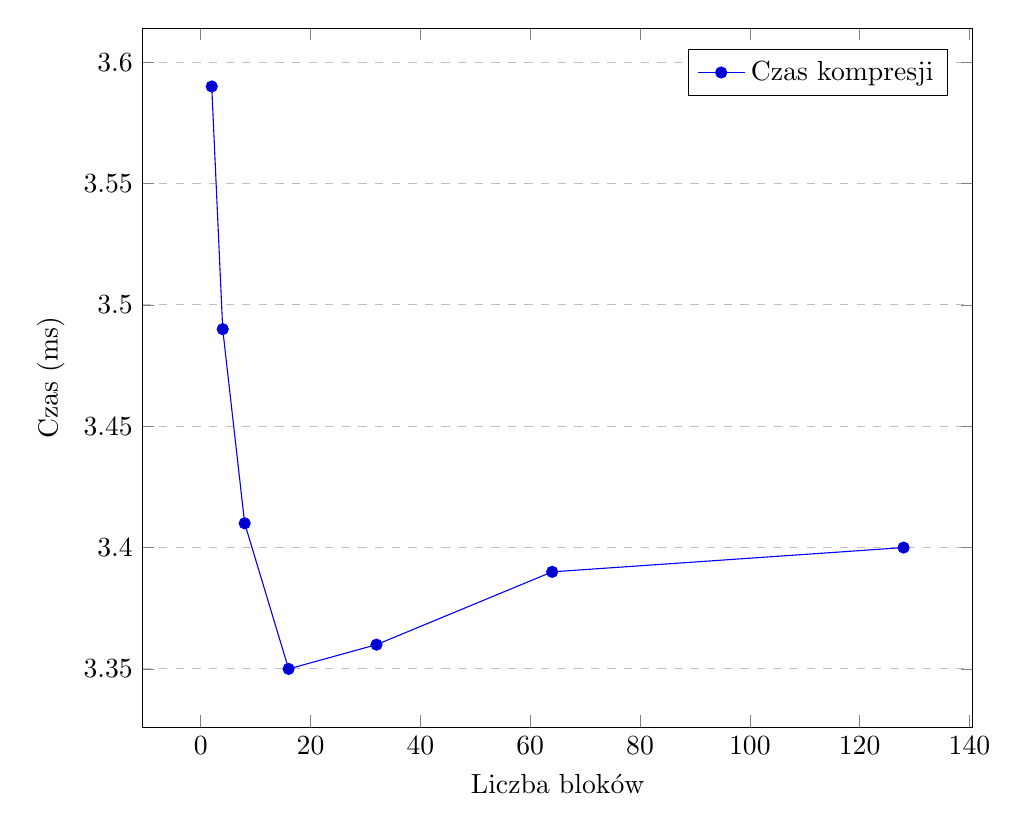
\begin{tikzpicture}
	\begin{axis}[
	    title style={yshift=2.5ex,},
	    align=center,
	    width=\textwidth,
		xlabel=Liczba bloków,
		ylabel=Czas (ms),
        ymajorgrids=true,grid style=dashed,
        legend pos=north east
        ]
        \addplot coordinates {
            (2, 3.59)
            (4, 3.49)
            (8, 3.41)
            (16, 3.35)
            (32, 3.36)
            (64, 3.39)
            (128, 3.4)
        };
        \legend{Czas kompresji}
    \end{axis}    
\end{tikzpicture}
\end{figure}

Po przeprowadzeniu testów można zauważyć zależność czasu kompresji od liczby bloków zbliżoną do logarytmicznej. Algorytm wykonał się najkrócej dla liczby bloków równej 16. Dla mniejszych liczb czas wykonania malał, natomiast dla większych rósł.\newline

\newpage
Podczas testowania wpływu wielkości plików na czas wykonywania algorytmu przyjęto następujące założenia:
\begin{itemize}
    \item 2 bloki,
    \item 32 wątki.
\end{itemize}

\begin{figure}[H]
\centering
\caption{Czas wykonywania algorytmu w zależności od rozmiaru pliku}
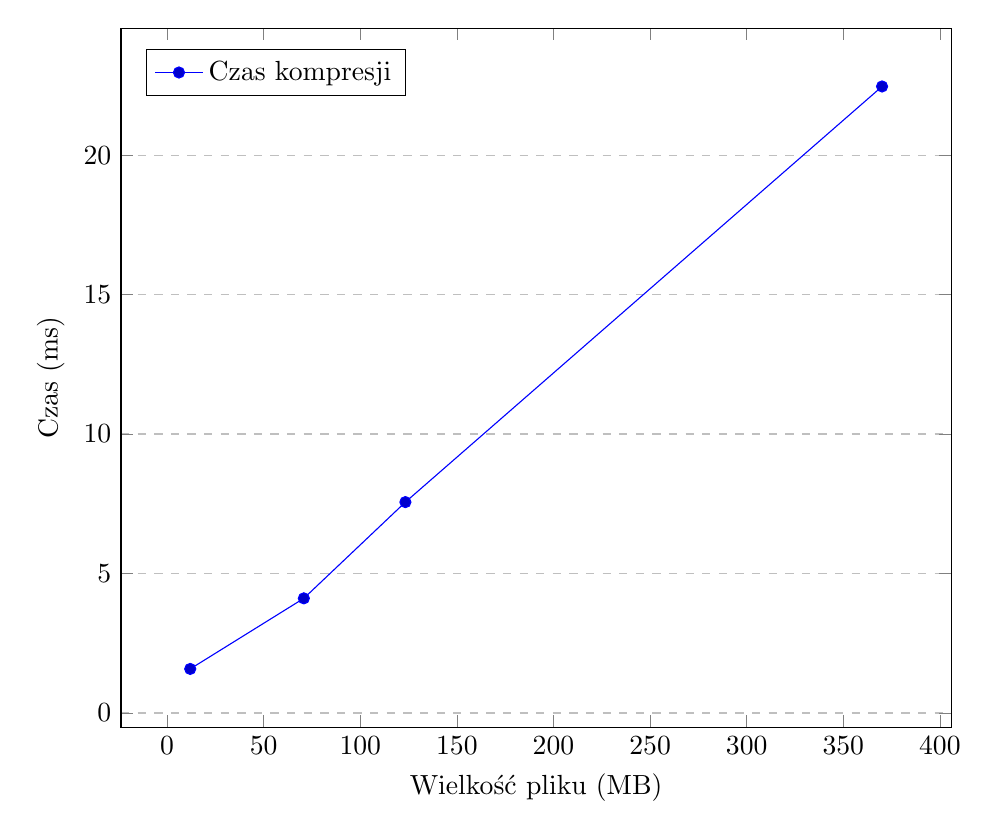
\begin{tikzpicture}
	\begin{axis}[
	    title style={yshift=2.5ex,},
	    align=center,
	    width=\textwidth,
		xlabel=Wielkość pliku (MB),
		ylabel=Czas (ms),
        ymajorgrids=true,grid style=dashed,
        legend pos=north west
        ]
        \addplot coordinates {
            (11.98, 1.58)
            (70.782, 4.11)
            (123.353, 7.56)
            (370.059, 22.46)
        };
        \legend{Czas kompresji}
    \end{axis}    
\end{tikzpicture}
\end{figure}

Z przedstawionego wyżej wykresu jednoznacznie wynika, że czas wykonania kompresji rośnie liniowo względem wielkości pliku wejściowego.
\newpage
\subsubsection{Wpływ zrównoleglenia zadań na czas obliczeń}
Podczas testowania wpływu liczby wątków na czas wykonywania algorytmu przyjęto następujące założenia:
\begin{itemize}
    \item 2 bloki dla wielu wątków,
    \item 1 blok dla pojedynczego wątku.
\end{itemize}
Testowane pliki posiadały rozmiary:
\begin{itemize}
    \item Mały - 11.98 MB,
    \item Średni - 70.782 MB,
    \item Duży - 123.353 MB,
    \item Bardzo duży - 370.059 MB.
\end{itemize}

\begin{figure}[H]
\centering
\caption{Czas wykonywania algorytmu dla małego pliku w zależności od liczby wątków}
\begin{tikzpicture}
	\begin{axis}[
	    title style={yshift=2.5ex,},
	    align=center,
	    width=\textwidth,
		xlabel=Liczba wątków,
		ylabel=Czas (ms),
        ymajorgrids=true,grid style=dashed,
        legend pos=north east
        ]
        \addplot coordinates {
            (2, 4.47)
            (4, 3.93)
            (8, 2.52)
            (16, 1.92)
            (32, 1.58)
            (64, 1.38)
            (128, 1.29)
            (256, 1.30)
            (1024, 1.30)
        };
        \addlegendentry{Czas kompresji dla wielu wątków}
        \addplot coordinates {
            (1, 0.91)
        };
        \addlegendentry{Czas kompresji dla 1 wątku}
    \end{axis}    
\end{tikzpicture}
\end{figure}

Z przedstawionego powyżej wykresu można odczytać, że czas kompresji małych plików przy użyciu jednego wątku jest znacznie krótszy od kompresji wielowątkowej. Zwiększanie liczby wątków pomaga osiągnąć lepsze wyniki, ale nie są one zbliżone do wyników pojedynczego wątku. Może to wynikać z faktu, że zatrzymywanie oraz wybudzanie wątków zajmuje czas. Różnica w czasie wykonywania algorytmu na 256 i 1024 wątkach jest niewielka.

\begin{figure}[H]
\centering
\caption{Czas wykonywania algorytmu dla średniego pliku w zależności od liczby wątków}
\begin{tikzpicture}
	\begin{axis}[
	    title style={yshift=2.5ex,},
	    align=center,
	    width=\textwidth,
		xlabel=Liczba wątków,
		ylabel=Czas (ms),
        ymajorgrids=true,grid style=dashed,
        legend pos=north east
        ]
        \addplot coordinates {
            (2, 5.59)
            (4, 5.50)
            (8, 5.36)
            (16, 5.23)
            (32, 4.11)
            (64, 3.75)
            (128, 3.58)
            (256, 3.59)
            (1024, 3.57)
        };
        \addlegendentry{Czas kompresji dla wielu wątków}
        \addplot coordinates {
            (1, 4.16)
        };
        \addlegendentry{Czas kompresji dla 1 wątku}
    \end{axis}    
\end{tikzpicture}
\end{figure}

Na przedstawionym wyżej wykresie widać, że pojedynczy wątek spisuje się gorzej dla średnich plików niż dla małych. W przypadku plików tej wielkości użycie 64 lub więcej wątków przyspiesza wykonywanie się algorytmu. Różnica w czasie wykonywania algorytmu na 128, 256 i 1024 wątkach jest niewielka.

\begin{figure}[H]
\centering
\caption{Czas wykonywania algorytmu dla dużego pliku w zależności od liczby wątków}
\begin{tikzpicture}
	\begin{axis}[
	    title style={yshift=2.5ex,},
	    align=center,
	    width=\textwidth,
		xlabel=Liczba wątków,
		ylabel=Czas (ms),
        ymajorgrids=true,grid style=dashed,
        legend pos=north east
        ]
        \addplot coordinates {
            (2, 10.59)
            (4, 10.21)
            (8, 9.77)
            (16, 8.42)
            (32, 7.56)
            (64, 6.57)
            (128, 6.28)
            (256, 6.32)
            (1024, 6.32)
        };
        \addlegendentry{Czas kompresji dla wielu wątków}
        \addplot coordinates {
            (1, 9.54)
        };
        \addlegendentry{Czas kompresji dla 1 wątku}
    \end{axis}    
\end{tikzpicture}
\end{figure}

Na przedstawionym wyżej wykresie widać, że algorytm kompresji wykonuje się znacznie szybciej dla 16 lub więcej wątków. Różnica w czasie wykonywania algorytmu na 128, 256 i 1024 wątkach jest niewielka.

\begin{figure}[H]
\centering
\caption{Czas wykonywania algorytmu dla bardzo dużego pliku w zależności od liczby wątków}
\begin{tikzpicture}
	\begin{axis}[
	    title style={yshift=2.5ex,},
	    align=center,
	    width=\textwidth,
		xlabel=Liczba wątków,
		ylabel=Czas (ms),
        ymajorgrids=true,grid style=dashed,
        legend pos=north east
        ]
        \addplot coordinates {
            (2, 141.59)
            (4, 129.21)
            (8, 64.77)
            (16, 40.42)
            (32, 22.46)
            (64, 22.71)
            (128, 21.70)
            (256, 27.83)
            (1024, 20.90)
        };
        \addlegendentry{Czas kompresji dla wielu wątków}
        \addplot coordinates {
            (1, 127.00)
        };
        \addlegendentry{Czas kompresji dla 1 wątku}
    \end{axis}    
\end{tikzpicture}
\end{figure}

Na ostatnim wykresie widać, że czas wykonywania algorytmu na wielu wątkach jest znacząco krótszy od tego wykonywanego na pojedynczym wątku. Można z tego wywnioskować, że im większy plik tym większy wpływ liczby wątków na czas kompresji. Różnica w czasie wykonywania algorytmu na 32, 64, 128, 256 oraz 1024 wątkach jest niewielka.

\subsection{Wnioski z testów i badań}
Z przeprowadzonych pomiarów wynika, że liczba bloków ma mały wpływ na czas wykonywania się kompresji. Istnieje jednak taki punkt, w którym czas osiąga minimum. Nie jest on jednak w pełni zależny od liczby bloków. Zwiększając liczbę bloków nie powodujemy poprawy szybkości wykonywania się algorytmu. Po przekroczeniu pewnego punktu możemy ten czas nawet pogorszyć.

Rozmiar pliku ma liniowy wpływ na czas wykonywania się algorytmu. Im większy plik, tym dłuższy czas kompresji.

Podczas testowania wpływu liczby wątków na czas wykonywania algorytmu zauważyliśmy, że w niektórych przypadkach czas kompresji na jednym wątku jest znacznie krótszy od kompresji wielowątkowej. Z wykresów można odczytać, że im większy plik tym bardziej wydajna jest kompresja na wielu wątkach. Dla małych plików (poniżej 20 MB) algorytm wykonuje się najszybciej na jednym wątku. Dla pozostałych wielkości czas kompresji jest krótszy dla wielu wątków, jednak nie dla każdej ich liczby. Istnieją liczby wątków, dla których kompresja jest mniej wydajna niż przy użyciu jednego wątku. Spowodowane jest to prawdopodobnie sposobem działania aplikacji wielowątkowych, ponieważ zatrzymywanie oraz wybudzanie wątków zajmuje czas. Im obszerniejszy plik tym liczba wątków osiągających lepsze wyniki niż pojedynczy wątek jest niższa. Z drugiej strony, gdy przekroczymy barierę pewnej ilości wątków algorytm się nasyci i nie zauważymy już przyrostu wydajności.

%-------------------------------------------------------------------------
\newpage
\section{Podsumowanie}
% TODO - dopisać coś jeszcze (więcej tekstu)
Podczas przeprowadzania prób uruchomienia jąder CUDA za pomocą jCUDA pojawiały się błędy, które uniemożliwiły nam poprawne przeprowadzenie testów. Ze względu na niezbyt obszerną dokumentację nie udało się ich rozwiązać. Zmusiło nas to do zmiany podejścia i zaimplementowania algorytmu kompresji przy użyciu języka C++ oraz zestawu narzędzi CUDA. Dopiero wtedy udało nam się przeprowadzić potrzebne testy.

\newpage
\bibliographystyle{unsrt}
\bibliography{references}

\end{document}
